\documentclass[10pt,a4paper]{article}
\usepackage[a4paper, top=2cm, bottom=1.5cm, left=1.5cm, right=1.5cm]{geometry} % Задать размеры полей.
\usepackage[warn]{mathtext} % Русские символы в формулах. Нужно писать до пакета babel. Указывает, что в формулах используются символы кириллицы, которые по умолчанию печатаются прямым шрифтом.
\usepackage[T2A]{fontenc}
\usepackage[utf8]{inputenc}
\usepackage[russian]{babel}
\usepackage{amsmath}
\usepackage{amssymb}
\usepackage{graphicx}
%\usepackage{floatrow}
\usepackage{booktabs}
\usepackage{wrapfig}
\usepackage{fancyhdr}
\usepackage{multicol}
\usepackage{xcolor}

\usepackage{float}
\usepackage{multirow}

\usepackage{subfigure}

% Объявляем новую команду для переноса строки внутри ячейки таблицы
\newcommand{\specialcell}[2][c]{%
	\begin{tabular}[#1]{@{}c@{}}#2\end{tabular}}

\newcommand{\figref}[1]{(См. рис. \ref{#1})}
\newcommand{\secref}[1]{(См. раздел. \ref{#1})}

\newcommand{\angstrom}{\text{\normalfont\AA}}
\newcommand{\e}[1]{\text{$\cdot10^{#1}$}}
\newcommand{\m}{\; м}
\newcommand{\mm}{\; мм}
\newcommand{\um}{\; мкм}
\newcommand{\A}{\; А}
\newcommand{\V}{\; В}
\newcommand{\uV}{\; мкВ}
\newcommand{\cels}{\; ^\circ С}

\pagestyle{fancy}
\fancyhead{}
\fancyhead[L]{\small Дедков Д.А., Маслов А.С., Исследование эффекта Комптона. МФТИ, 2023 г.}
\fancyhead[R]{}
\fancyfoot[C]{\thepage}

\renewcommand{\cot}{\text{ctg}}

\author{\normalsize Дедков Денис, Маслов Артём \\
	\normalsize группа Б01-108а \\
	\normalsize 06.11.2023}
\date{}

\title{
	\Large Исследование эффекта Комптона. \\ 
}

\begin{document}
\maketitle
	
	\subsection*{Цель и задачи работы:}
	\begin{enumerate}
		\item С помощью сцинтилляционного спектрометра исследуется энергетический спектр $\gamma$-квантов, рассеянных на графите. Определяется энергия рассеянных $\gamma$-квантов в зависимости от угла рассеяния, а также энергия покоя частиц, на которых происходит комптоновское рассеяние.
	\end{enumerate}
	
	\subsection*{Описание экспериментальной установки}
	
	Схема экспериментальной установки приведена на рисунке \ref{img:exp_scheme}:
	\begin{figure}[H]
		\centering
		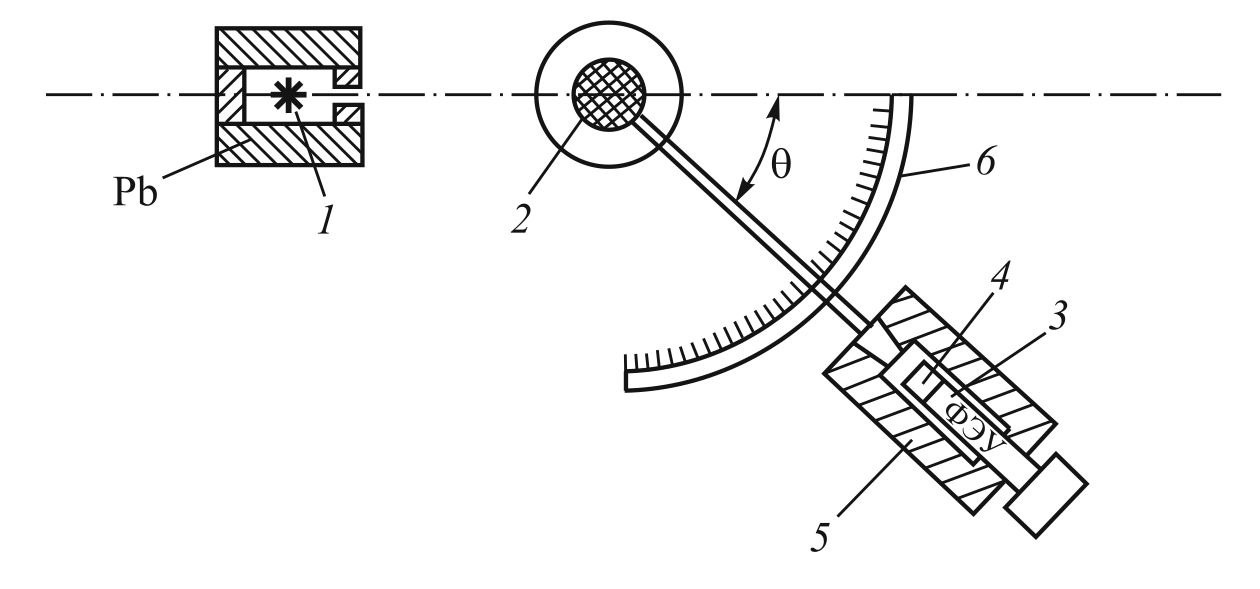
\includegraphics[width=0.45\textwidth]{img/exp_scheme.png}
		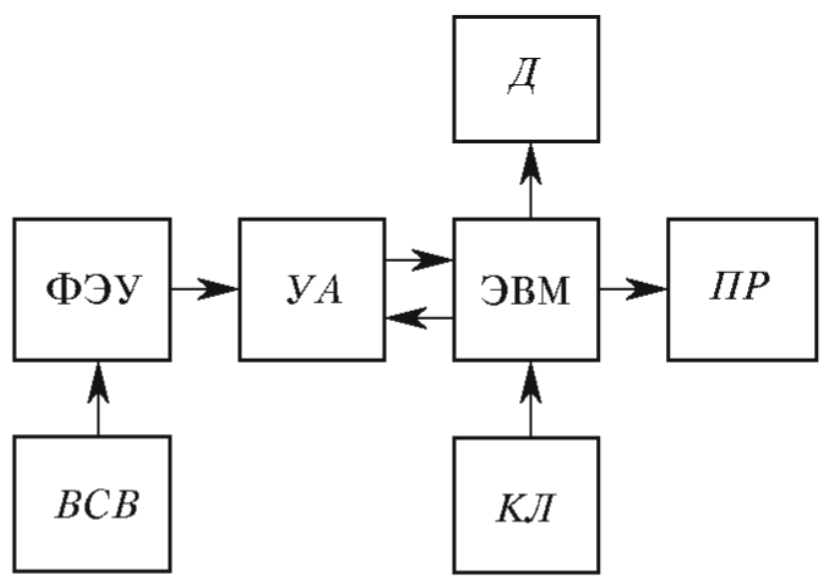
\includegraphics[width=0.45\textwidth]{img/prin_scheme.png}
		\caption{Слева схема экспериментальной установки. Справа принципиальная схема измерительного комплекса.}
		\label{img:exp_scheme}
	\end{figure}

	Источником излучения 1 является ${}^{137}Cs$, испускающий гамма-кванты с энергией 662 кэВ. Источник излучения помещён в толстостенный свинцовый контейнер с коллиматором. Сформированный коллиматором узкий пучок гамма-лучей попадает на графитовую мишень 2, которой является цилиндр высотой 100 мм и диаметром 40 мм. Кванты, испытывающее комптоновское рассеяние в мишени, регистрируются сцинтилляционным счётчиком (4-5). Счётчик состоит из фотоэлектронного умножителя ФЭУ 3 и сцинтиллятора 4. Сцинтиллятором служит кристалл $NaI(Tl)$ цилиндрической формы высотой 40 мм, диаметром 40 мм, его выходное окно находится в оптическом контакте с фотокатодом ФЭУ. Сигналы, возникающие на аноде ФЭУ подаются на ЭВМ. ФЭУ расположен в светонепроницаемом блоке, закреплённом на штанге, которая может вращаться в горизонтальном направлении. Угол поворота измеряется по лимбу 6.
	
	\subsection*{Оборудование и приборы}
		
	Стенд с экспериментальной установкой номер $1.2._3$.
	\begin{enumerate}
		\item Лабораторная установка для исследования абсолютной активности кобальта-60 $ЛУ-4.3-2$. Заводской номер №1513. Инвентарный номер №410134174169.
				
		\item Высоковольтный блок питания. Инвентарный номер №410134125762.
		
		\item Блок оцифровки и обработки данных. Инвентарный номер №410136146940.
		
		\item Сцинтилляционный детектор Радек. Инвентарный номер №4013.
				
		\item Радиоактивный источник в свинцовой оболочке ${}^{137}Cs$. Энергия гамма-квантов 662 кэВ. Инвентарный номер №11010712637.
	\end{enumerate}
	
	\subsection*{Первичные экспериментальные данные}
	
	Первичные экспериментальные данные приведены в таблице:\\
	\begin{center}
		\begin{tabular}{ccccc}
\toprule
$\theta, ^\circ$ & $\sigma_{\theta}, ^\circ$ & $N$, кан. & $\sigma_N$, кан. & $\Delta N$, кан. \\
\midrule
0 & 3 & 923 & 5 & 89 \\
10 & 3 & 812 & 5 & 79 \\
20 & 3 & 778 & 5 & 95 \\
30 & 3 & 790 & 5 & 91 \\
40 & 3 & 743 & 5 & 89 \\
50 & 3 & 614 & 5 & 83 \\
60 & 3 & 558 & 5 & 82 \\
70 & 3 & 482 & 5 & 78 \\
80 & 3 & 431 & 5 & 65 \\
90 & 3 & 400 & 5 & 56 \\
100 & 3 & 371 & 5 & 53 \\
110 & 3 & 327 & 5 & 49 \\
120 & 3 & 313 & 5 & 48 \\
\bottomrule
\end{tabular}

	\end{center}

	
	$\theta$ -- угол между исходным направлением гамма-квантов и направлением наблюдения, $N$ -- номер канала, зарегистрировавшего наибольшее число частиц (фотопик), $\Delta N$ -- ширина пика по половине высоты. Оценим погрешности измерения первичных экспериментальных данных. Погрешность измерения угла отклонения определяется геометрией установки $\sigma_\theta = \frac{\text{Ширина детектора}}{\text{Расстояние до детектора}} \approx 3^\circ$. Погрешность, связанная с конечностью каналов АЦП (всего 1024 канала, ошибка попадания в канал $\pm 0.5$ каналов): $\varepsilon = \frac{0.5}{1024} = 0.05 \%$. Из-за шума, связанного с Пуассоновским распределением количества зарегистрированных частиц, возникает погрешность определения положения фотопика, которая оценивается как $\sigma = \pm 5$ каналов. Итоговая погрешность определения положения фотопика $\sigma_ф = \pm 5$ каналов и одинакова для всех измерений.
	
	\subsection*{Обработка экспериментальных данных}
	
	Согласно теории, распределение рассеянных на углы $\theta$ гамма-квантов вследствие комптоновского рассеяние определяется соотношением: 
	$$
	\frac{1}{\varepsilon(\theta)} - \frac{1}{\varepsilon_0} = 1 - \cos \theta
	$$
	Номер канала, зарегистрировавший гамма-квант пропорционален его энергии, тогда
	$$
	\frac{1}{N(\theta)} - \frac{1}{N(0)} = A (1 - \cos \theta)
	$$
	Построим график зависимости $1/N(\theta)$ от $(1 - \cos \theta)$.\\
	\begin{figure}
		\centering
		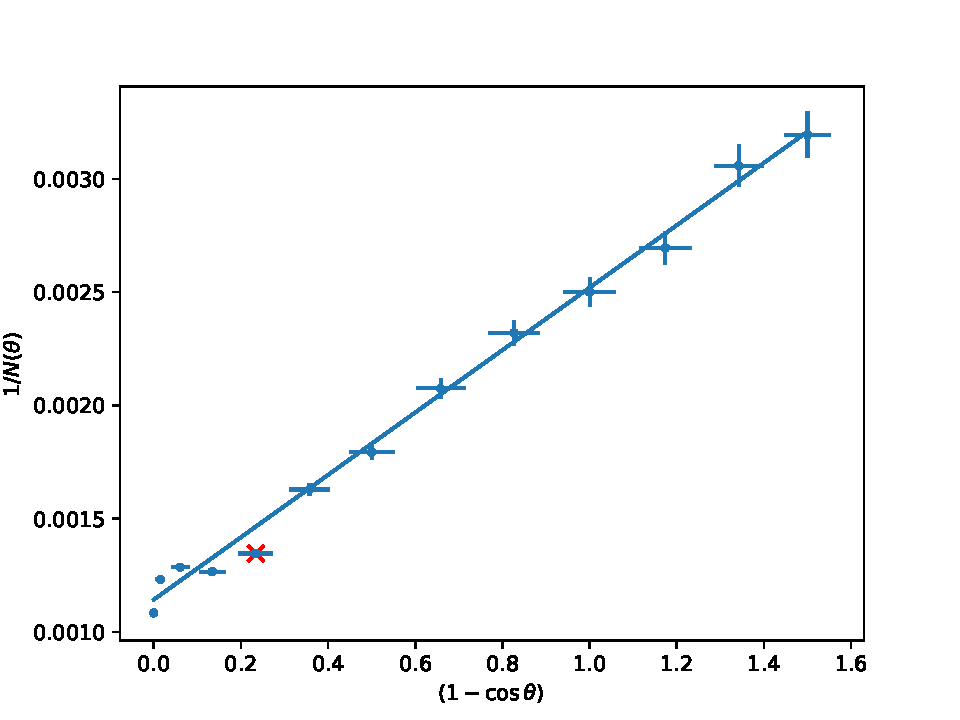
\includegraphics[width=0.6\textwidth]{gen/plot1.pdf}
		\caption{График зависимости $1/N(\theta)$ от $(1 - \cos \theta)$.}
	\end{figure}

	По пересечению графика с осью ординат определим $N(0)$:
	$$N(0) = 846 \pm 11$$
	Погрешность оценим по формуле косвенных измерений: 
	$$y_{аппрокс} = ax + b$$
	$$N(0) = \frac{1}{b}$$
	$$\varepsilon_{N(0)} = \frac{\sigma_b}{b}$$
	
	По пересечению графика с прямой $\cos \theta = 0$ определим $N(90)$:
	$$N(90) = 384 \pm 4$$
	Погрешность оценим по формулам: 
	$$y_{аппрокс} = ax + b$$
	$$N(90) = \frac{1}{b + a}$$ 
	$$\sigma_{N(90)} = \frac{1}{(a + b)^2}\sqrt{\sigma_b^2 + \sigma_a^2}$$
	
	Определим энергию покоя электрона, на котором происходило рассеяние гамма-квантов: \\
	$$
	mc^2 = E_\gamma \frac{N(90)}{N(0) - N(90)} = 550 \pm 16 \; кэВ
	$$
	где $E_\gamma = (662\pm1) кэВ$ -- энергия гамма-лучей, испускаемых источником. Оценим погрешность определения $mc^2$:\\
	$$\sigma_{mc^2} = \sqrt{(\frac{N(90)}{N(0) - N(90)} \sigma_{E_\gamma})^2 + (\frac{N(90) E_\gamma}{(N(0) - N(90))^2} \sigma_{N(0)})^2 + (E_\gamma \frac{N(0)}{(N(0) - N(90))^2}\sigma_{N(90)})^2}$$
	
	\subsection*{Обсуждение результатов и выводы}
	
	В работе был проверен закон комптоновского рассеяния:
	$$
	\frac{1}{\varepsilon(\theta)} - \frac{1}{\varepsilon_0} = 1 - \cos \theta
	$$
	Экспериментальные точки ложатся на прямую в пределах $2\sigma$.
	
	Определено значение энергии покоя электрона $$mc^2 = 550 \pm 16 кэВ$$. \\
	Табличное значение энергии покоя электрона $$mc^2_{табл} = 510.998 кэВ$$.
	
\end{document}